\chapter{Introduction}

Provenance as a concept has been around for a long time. It originally comes from the Latin word \textit{provenio}, meaning ``to come forth''. It's primary use is in the field of antiques where provenance is used to identify the authenticity and quality of something. For anyone with a backgruond in databases this term may also be fimilair as linking tuples in a query output to the reasons they exist.

In this paper the provenance we refer to is that of \textit{digital provenance}. It is a type of metadata representing the lineage of an object. Naively it can be compared to the information stored in revision history systems like that used in google docs\footnote{Google docs: \url{https://docs.google.com}} or version control
% TODO: git and mercurial links
systems such as git\footnote{GIT\: \url{}} or mercurial. These systems are usually limited to storing revisions as well as authorship. However extends beyond this by making it posible to store and ultimately trace what other things and activities led to a digital object been in its current state.

Provenance has the potential for usefulness in many different fields. The foremost and focus of this paper is the field of personal data management, allowing users to understand how their data is used. Often when a user chooses to share their personal data it is aggregated, anonymised or passed through any number of functions. By exploring provenance users have the ability to understand exactly how much and in what state their personal data is used.

An example to illistrate this point. Alice has a report that describes her current fitness level as well as outlining possible improvements. Viewing the provenance of
% TODO: Fitbit and Withings footnotes
this report shows which sources have been used (e.g. Fit-Bit data to track steps, Withings scale to track weight) and what processes analysed them. In this case it could show that Alice's fitness report was generated using step data from her FitBit data, passed through a summarisation process that summarises 15 minute interval data into daily steps. This shows tracing of lineage backwards in time, it is also possible to trace information forward, possibly in the case of errors in data. Alice remembers that she lent her FitBit to a friend to try for a week, causing errors in her data. Provenance would allow tracing of the errenous information forward to see what other processes and entities it effected and would need to be corrected.

Provenance is also potentially useful in any field where the lineage of an object needs to be stored. This could be extended to digital records of antiques or artwork. This would also be useful in data warehouse systems where information about data transformations as well as origin are stored. There is also research into storing provenance in
% TODO: reference to block chains
block-chains or similar systems to prevent medling of historical data where it to be used in high risk systems such as banks or accounting systems.

Early provenance systems stored provenance information in a variety of different flat
% TODO: prov reference
file formats. Since 2013, the PROV specification has provided a generic model for storing provenance with a number of serialisations (PROV-N, XML, JSON and RDF). PROV identifies provenance elements as three main concepts:

\begin{itemize}
	\item Entities: Physical, digital, conceptual objects
	\item Activities: Elements that cause an entity to come into existence
	\item Agents: Someone or something that can be assigned responsibility for an activity taking place.
\end{itemize}

The industry standard for representing these concepts is on an acyclic graph. An example of this with each of the three main concepts can be see in Figure~\ref{fig:key-concepts}.

\begin{wrapfigure}{r}{0.5\textwidth}
	\centering
	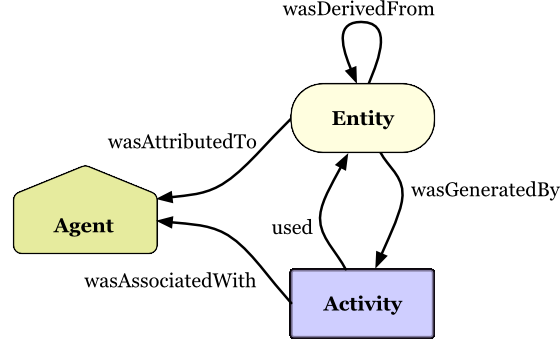
\includegraphics[width=\linewidth]{key-concepts}
	\caption{Key Concepts and relationships from the PROV standard displayed in a labelled acyclic graph.}
	\label{fig:key-concepts}
\end{wrapfigure}

Provenance can be stored in a variety of different granularity's and levels. The main three levels or provenance are system-level, application-level and network level. System level provenance is the lowest level and will often capture operating system activities such as which application ran at what to point to affect a piece of data. Application level provenance is limited to a single application, and will often capture information directly related to the user using that application. Network provenance captures information via network switches and stores lineage originating from multiple machines. These three levels are quire broad and do not cover all use cases but they do give a good point for starting discussion and comparing provenance capture tools. Provenance is also captured at different levels of granularity. Using the example of Alice as above, a system may capture information about her step data at the smallest granularity: how many steps every 15 minutes, or it may store the information at a larger granularity: aggregating step data daily.

As you can see in Figure~\ref{fig:key-concepts} provenance graphs are most often represented as directed acyclic graphs
% TODO: Novel provenance representation citing
although there has been some other novel approaches. The main problem we discuss is  provenance can become incredibly large, particularly in the case of OS level recording as it is usually at a low granularity so a lot of data is been recorded in a small time. Because provenance is inherently historical it is forever growing in size (as of yet there's no standard for going back and ``compressing'' history,) this means even  provenance captured as a high granularity will monotomiously grow and can become a graph with thousands or millions of nodes. This quickly becomes a
% TODO: usability studies chapter cite
usability problem as users can't visually digest such large graphs (results for usability studies in section x show that users are even put off by graphs with as little as 30 nodes).

What we describe in this paper is a process of simplifying graphs by clustering nodes into single composite nodes. A part from simplifying the graph and presenting less objects on screen, this also allows users to control what information is seen by other people or highlight particular concepts as seen in section x.
